\section{Partie 2: Parallélisation de NTMIX}


Comme vu dans l'introduction, l'objectif est de pouvoir exécuter cette application sur un maillage de taille conséquente ($\approx 10^9$ points) ce qui est impossible de faire sur un unique processeur; en effet, pour chaque point d'un maillage, au moins 5 variables conservatives doivent être stockées (densité, vitesses et l'énergie). Chacune de ces variables sont des nombres à virgule flottante en double précision (méthode utilisée pour représenter les nombre réels en informatique) occupant 8 octets. L'espace nécessaire pour stocker ces variables serait de $10^9 \times 5 \times 8 \approx 37.25$ Go, auquel il faudrait ajouter les $7.45$ Go par espèce chimique. Sachant qu'un des tests qui sera utilisé possédera 27 espèces, nous arrivons à un total de $37.25+27 \times 7.45\approx 238.42$ Go seulement pour stocker les variables nécessaires à la simulation auxquelles il faudrait encore ajouter les tableaux de travail.





De plus, la charge de calcul serait colossale; j'ai mesuré le temps par points de la version séquentielle (\ref{}). On peut voir que pour un maillage d'environ 15 millions de points, le temps par point est de 4 $\mu$s. Dans le cas optimiste où la courbe n'augmenterait pas, un pas de temps pour $10^9$ points durerait $10^9\times4\times10^{-6}=4000$s ($\approx$ 1 heure 7 minutes). Une simulation de 10000 pas de temps durerait donc $4000\times10^4$ secondes $\approx$ 463 jours. (TODO: revoir le calcul avec les infos de bench)

\subsection{Décomposition de domaine}
\paragraph{}Il est donc impératif de diviser la charge de travail ainsi que la mémoire utilisée par le programme afin d'arriver à des nombres plus raisonnables. 
Pour cela, il est possible de partitionner le domaine de la simulation en plusieurs sous-domaines, plus petits, et de réaliser les calculs de chaque sous-domaine sur des processeurs différents. MPI (\textit{Message Passing Interface}) décrit une librairie permettant de définir des topologies virtuelles et les transferts de données entre les nœuds d'une telle topologie et permettra donc de diviser le domaine selon une grille cartésienne de processus. Chaque case d'une telle topologie calculera une petite partie de la solution globale mais pourra le faire en parallèle des autres. La figure \ref{fig:globaldom} représente un domaine en 2D avec en bleu ses bordures physiques. La figure \ref{fig:globaldom} montre un partitionnement de ce domaine en 4 sous-domaines, chacun possédant de nouvelles bordures.

Concrètement, chaque nœud de la topologie exécutera le même code mais sur des données différentes.
\begin{figure}[h!]
  \centering
  \begin{subfigure}[b]{0.5\textwidth}
    \centering
    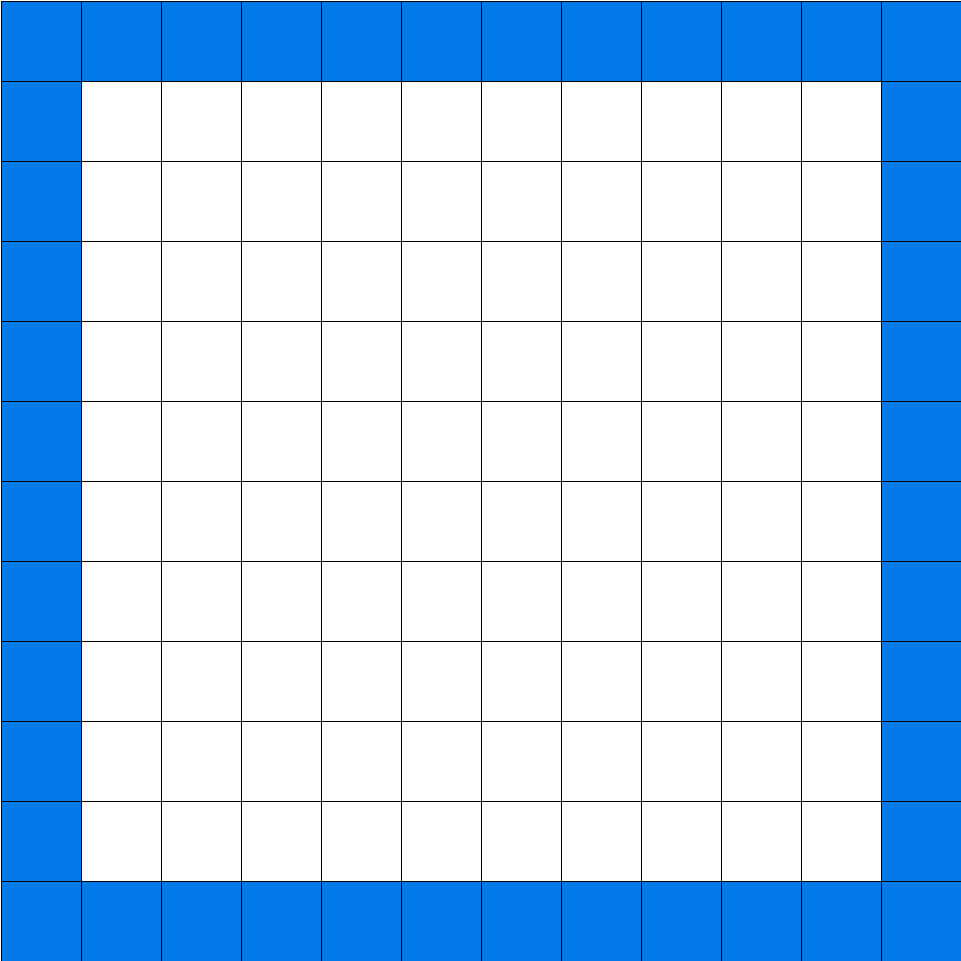
\includegraphics[scale=0.15]{figures/globaldomain.png}
  \caption{\label{fig:globaldom}Domaine complet}
  \end{subfigure}%
  ~
  \begin{subfigure}[b]{0.5\textwidth}
    \centering
    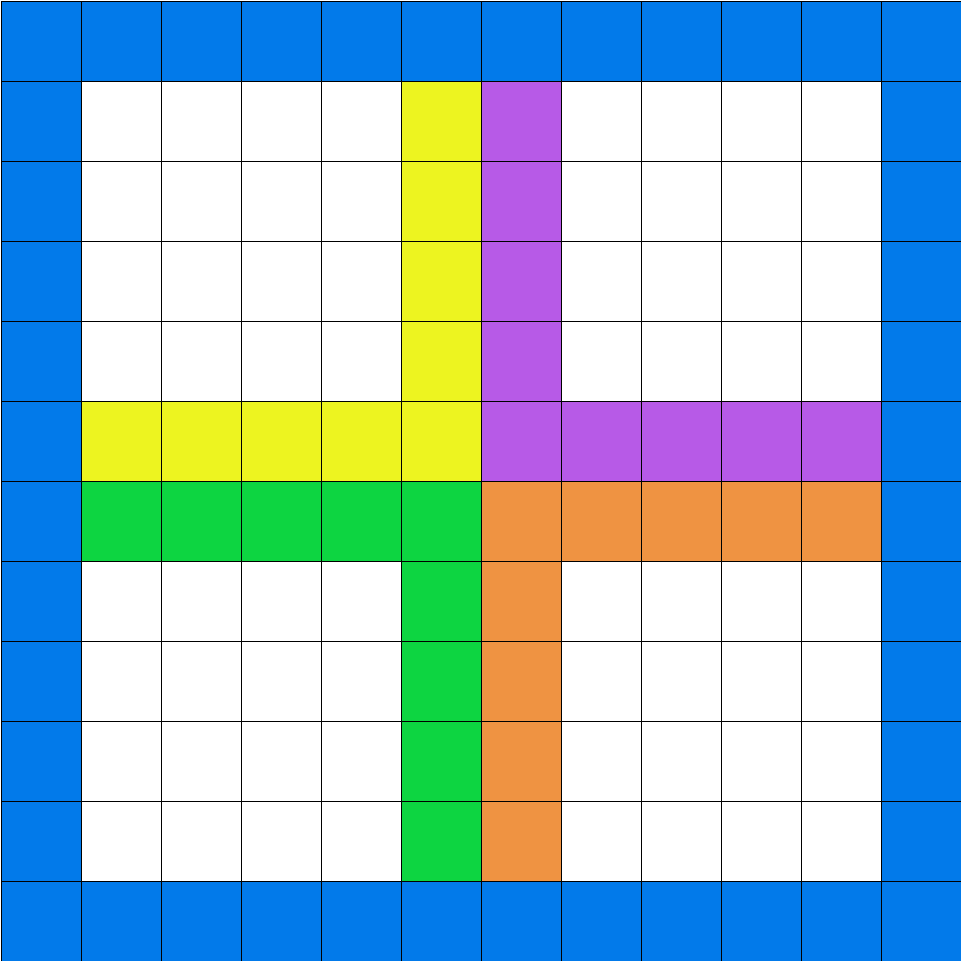
\includegraphics[scale=0.15]{figures/partitionnedomain.png}
  \caption{\label{fig:partdom}Domaine partitionné}
  \end{subfigure}
  \caption{\label{fig:dom}Partitionnement du domaine}
\end{figure}

Dans le cas de NTMIX, il y a 2 cas différents pour la décomposition d'un domaine:
\begin{itemize}
\item le cas périodique: ce cas, utilisé pour éliminer les problèmes décrits en section \ref{sec:nsbc}, ne possède donc pas de bordures physiques, le recouvrement doit également se produire sur les processus se trouvant en bord de la topologie.
\item le cas non-périodique: dans ce cas les propriétés physique des bordures sont traitées et les processus se trouvant en bord de domaine ne possèdent donc pas de région d'overlapping.
\end{itemize}


\subsection{Recouvrement de domaine}
Cependant, chaque processus ne peut pas travailler de manière totalement indépendante. En effet, une méthode compacte est utilisée pour calculer les gradients des différents champs \cite{Hirsch:1988:NCI:63653}. Une telle méthode implique que le gradient en un point est dépendant des valeurs de tous les autres points du champ. Comme on peut le voir sur la figure \ref{fig:depdom}, après le partitionnement du domaine, les points se trouvant sur les bordures internes (bordures entre processus) manque d'information pour réaliser les calculs. Concrètement, les sous-domaines devront s'échanger les données présentes sur leurs bordures. 
%Pour cela, je testerai 2 méthodes avant de comparer leurs performances respectives.

%\paragraph{Méthode avec cellules fantômes}
 \paragraph{}Avec MPI, des communications devront se faire pour échanger ces données et il est nécessaire de réduire au maximum leur nombre. Pour cela, j'ai agrandi les sous-domaines en ajoutant des cases qui seront destinées au stockage d'une copie des données des domaines adjacents. Ces cases, appelées ``cellules fantômes'', sont représentées en gris sur la figure \ref{fig:depdomover} (ici la zone d'overlapping est représentée par une seule case pour la clarté du schéma mais la taille de cette zone peut varier).
Cette méthode permet donc de limiter le nombre de communications entre les processus mais des calculs sont répliqués sur plusieurs processus; en effet les points contenus dans les zones grisées seront calculées pour préparer les variables avant le calcul des gradients 2 fois.



\begin{figure}[h!]
  \centering
  \begin{subfigure}[b]{0.5\textwidth}
    \centering
    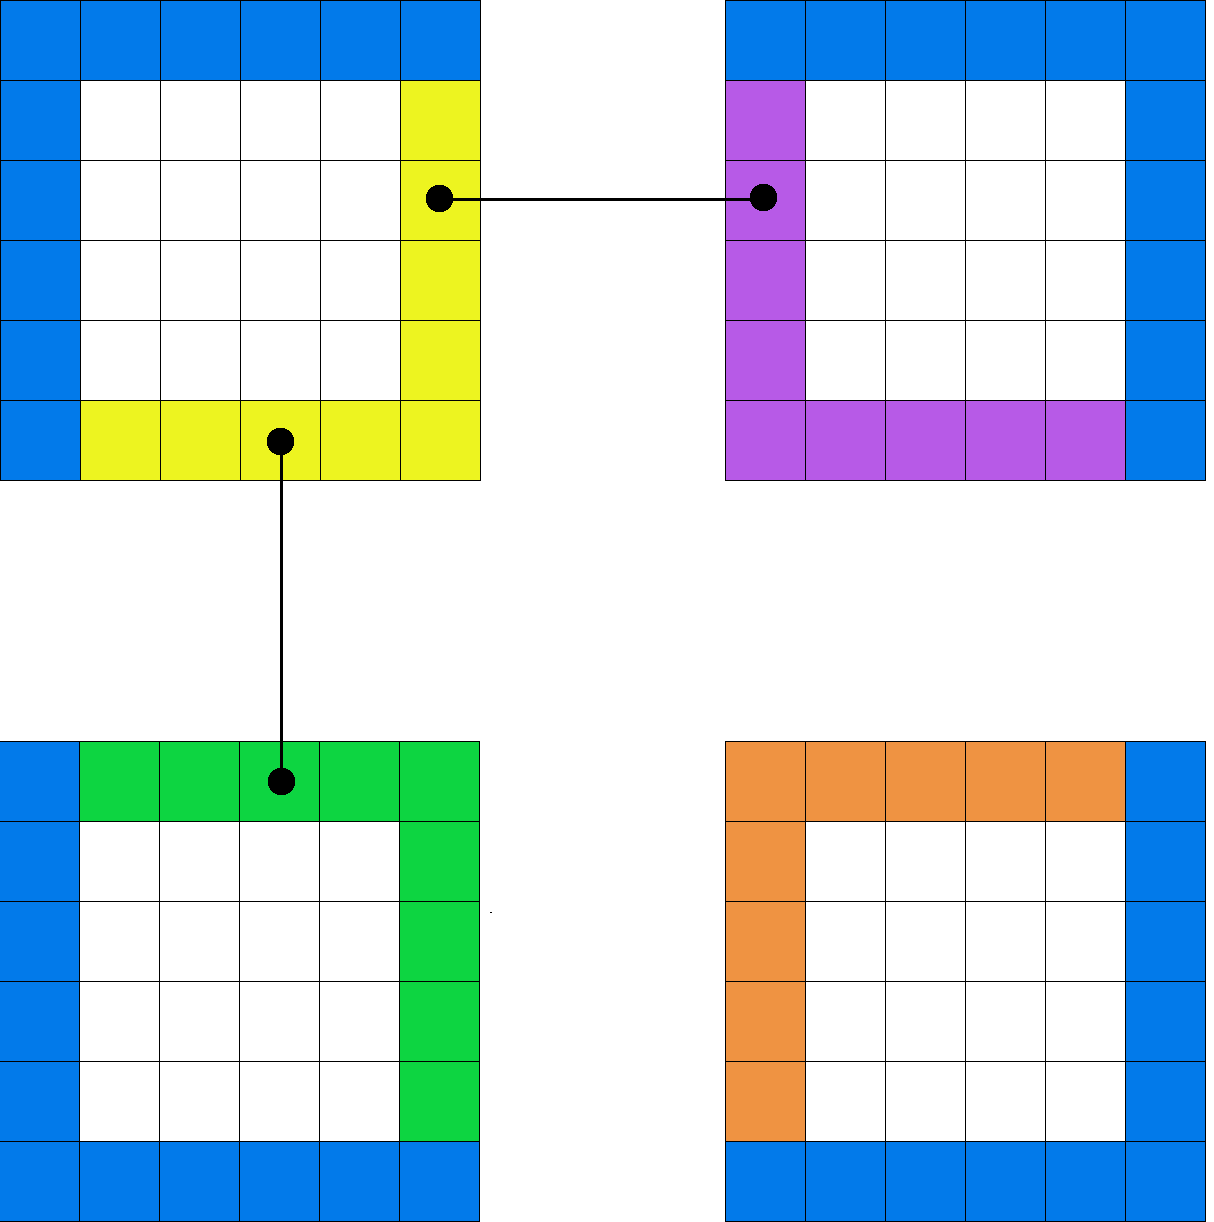
\includegraphics[scale=0.15]{figures/depdomain.png}
  \caption{\label{fig:depdom} }
  \end{subfigure}%
  ~
  \begin{subfigure}[b]{0.5\textwidth}
    \centering
    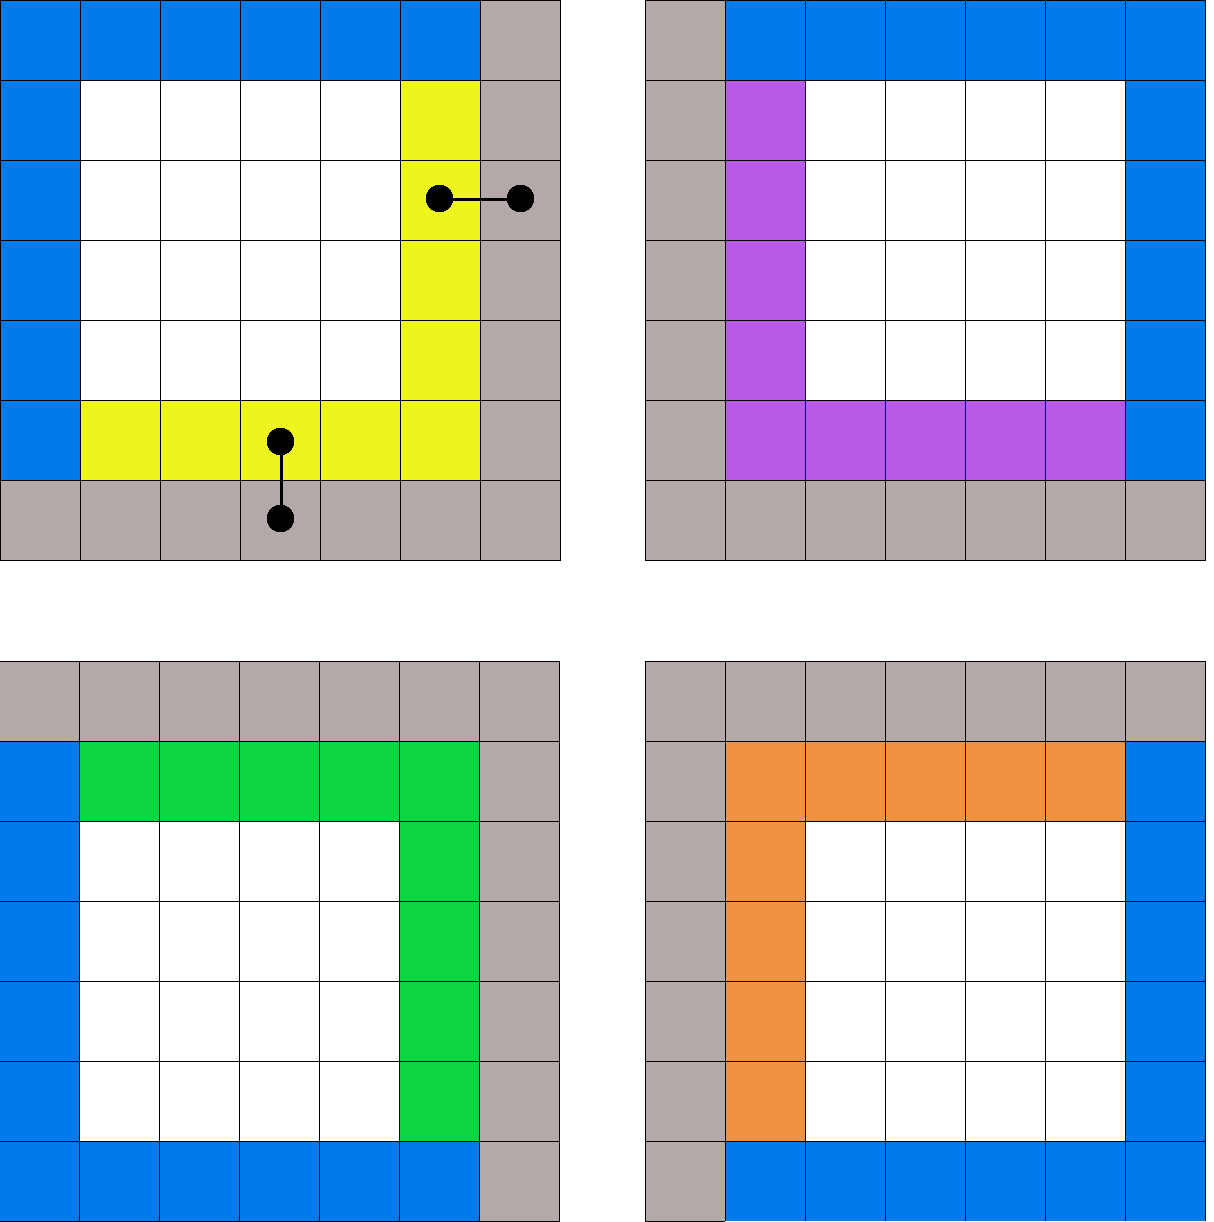
\includegraphics[scale=0.15]{figures/depdomain-overlap.png}
  \caption{\label{fig:depdomover} }
  \end{subfigure}
  \caption{\label{fig:domdep}Overlapping entre les sous-domaines}
\end{figure}


%\paragraph{Méthode sans réplication de calcul}
%La seconde méthode consiste à ne pas répliquer les calculs sur plusieurs sous-domaines. Pour cela, les zones d'overlapping ne sont donc pas créées et les échanges de données se font seulement au moment du calcul des gradients. Les sous-domaines reçoivent ainsi les données nécessaires quand ils en ont besoin. Cette méthode réduit donc les calculs réalisés par chacun des sous-domaines mais augmente grandement la quantité de communications.

%\paragraph{}J'ai donc ajouter ces méthodes au programme pour pouvoir comparer leurs performances respectives. La première méthode a l'avantage de reduire la fréquence des communications en dupliquant des calculs sur plusieurs processus (augmentant donc le côut de ceux-ci).


\subsection{Communications}
%Le fait que les sous-domaines issus de la décomposition ne soient pas totalement indépendant implique que des points de synchronisation doivent se mettre en place entre eux. En effet, il es nécessaire que de l'information transite entre les sous-domaines pour le calcul du pas de temps ou pour l'échange des cellules fantômes.

\subsubsection{Calcul du pas de temps}
Dans la version séquentielle de NTMIX, un pas de temps maximum, permettant de garantir la stabilité de la simulation, est calculé sur l'ensemble du domaine.
Dans la version parallèle, chaque sous-domaine calcule son pas de temps maximal et une opération de réduction est utilisée pour trouver le minimum global. Elle permet de trouver le pas de temps minimal entre tous les sous-domaines et de le distribuer sur tous les processus.

%\paragraph{}Dans la version séquentielle, un pas de temps maximal est calculé dans le but d'assurer la stabilité de l'algorithme. Ce calcul est donc dépendant de l'ensemble du domaine. Dans la version parallèle, chaque processus devra donc calculer le pas de temps maximal de son sous-domaine et le communiquer aux autres afin de trouver le pas de temps global (opération de réduction).

\subsubsection{Transfert des cellules fantômes}


%Les 2 méthodes permettant le transfert des données entre les sous-domaines présentées dans la section précédente impliquent des communications différentes; autant dans la quantité de données échangées et dans 


Du fait de la discrétisation du temps dans la simulation, une méthode de Runge-Kutta est utilisée pour réaliser la dérivation temporelle. C'est une méthode itérative; une première estimation de la solution est utilisée pour calculer une seconde estimation plus précise, et ainsi de suite \cite{Hirsch:1988:NCI:63653}. Dans NTMIX, 3 itérations sont réalisées à chaque pas de temps.
Il est donc nécessaire que les transferts des zones d'overlapping se fassent avant chaque appel à ces itérations afin que le calcul de l'intégration puisse se faire. Pour cela, j'ai créé une fonction update qui est appelée avant chaque itération de RHS (algo \ref{algo:time_step}).
%Dans RHS, toutes les variables conservatives subissent le calcul. 

\begin{algorithm}
  \caption{time\_step}
  \label{algo:time_step}
  \begin{algorithmic}
     \STATE {Call Update}
     \STATE {Call RHS(1)} 
     \STATE {Call impose\_boundary\_conditions}
     \STATE {Call Update}	
     \STATE {Call RHS(2)} 
     \STATE {Call impose\_boundary\_conditions}
     \STATE {Call Update}
     \STATE {Call RHS(3)} 
     \STATE {Call impose\_boundary\_conditions}
  \end{algorithmic}
\end{algorithm}



Chaque processus doit envoyer ses bordures à tous ses voisins dans la topologie virtuelle (fig. \ref{fig:comm}). MPI fournit une fonction permettant de réaliser ce type de communication; MPI\_Neighbor\_alltoallv. Pour l'utiliser, il faut préparer un buffer qui contiendra les données à envoyer à chacun de ses voisins(fig. \ref{fig:neighbor_pos}). La fonction gère automatiquement la répartition des buffers à envoyer aux voisins selon leur disposition sur la topologie. Après l'appel à cette fonction, le buffer de réception contient les données de tous les voisins autour d'un processus. Il ne reste plus qu'à stocker les variables reçues à leur place. 

\begin{figure}[h!]
  \centering
  \begin{subfigure}[b]{0.5\textwidth}
    \centering
     \fbox{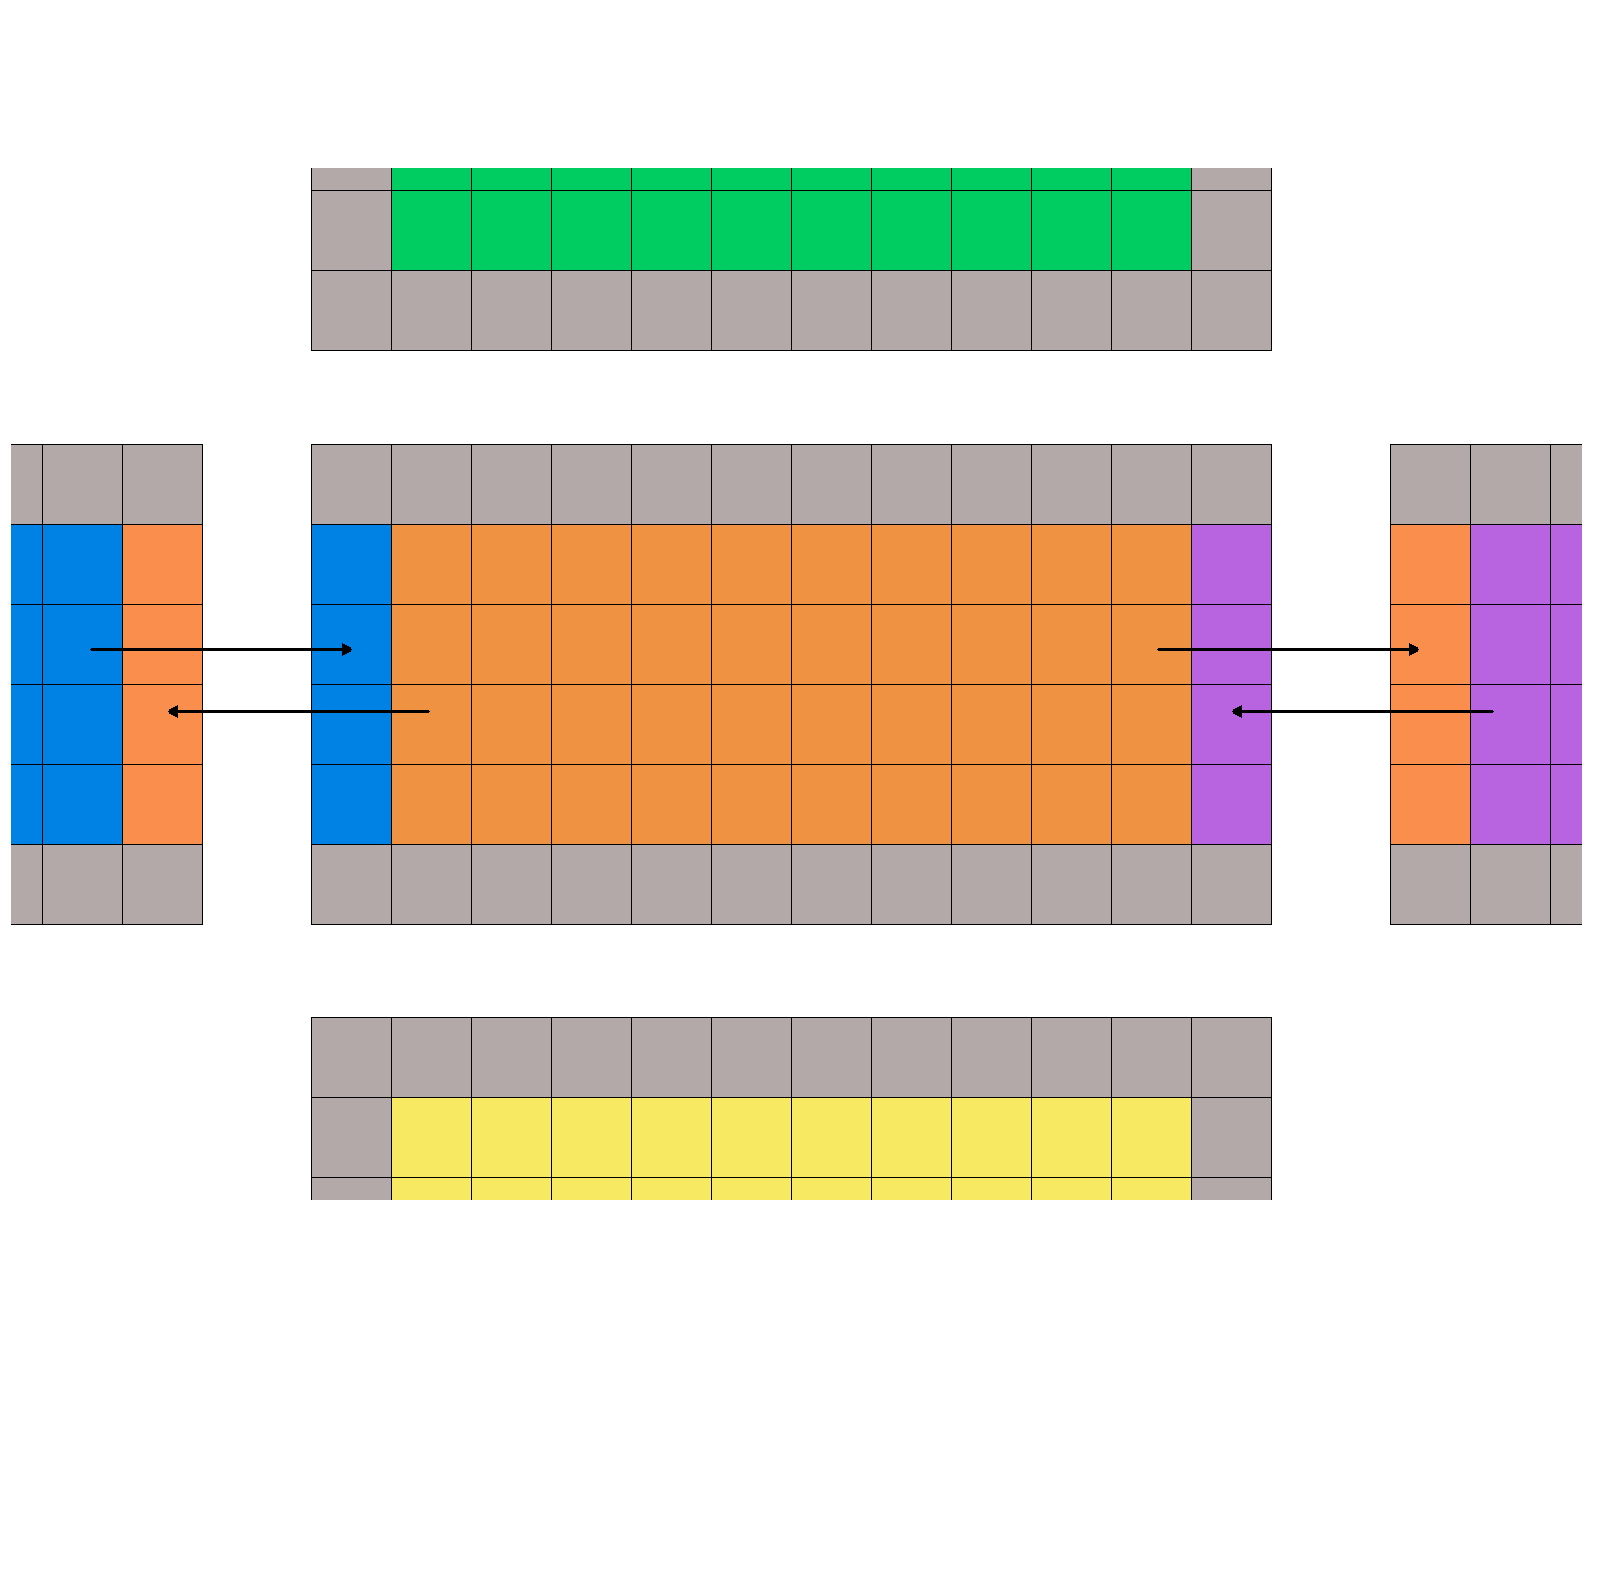
\includegraphics[scale=0.12]{figures/comms_dim1.png}}
  \caption{\label{fig:comm_dim1}}
  \end{subfigure}%
  ~
  \begin{subfigure}[b]{0.5\textwidth}
    \centering
     \fbox{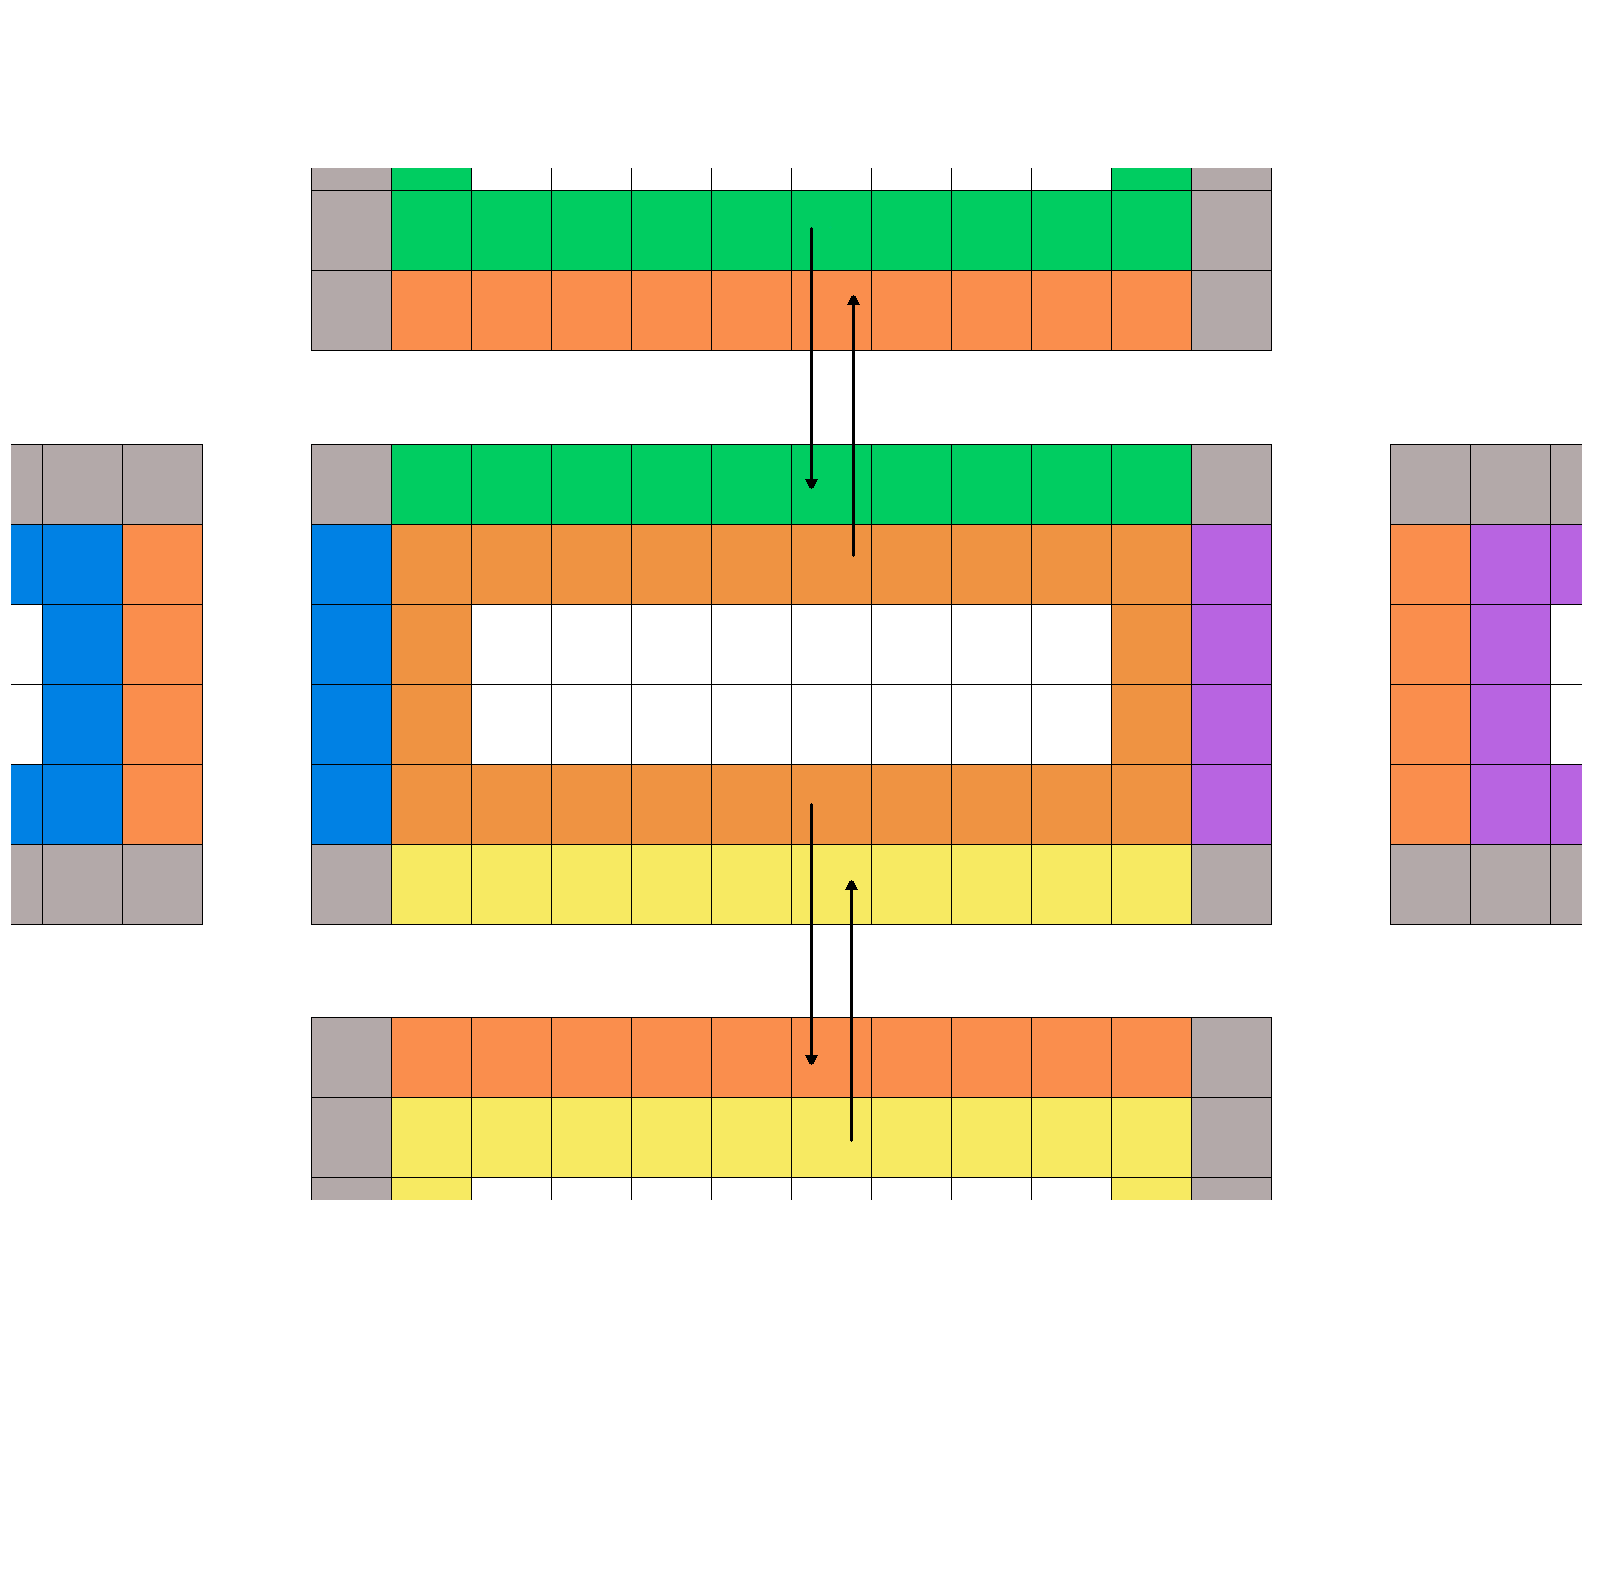
\includegraphics[scale=0.12]{figures/comms_dim2.png}}
  \caption{\label{fig:comm_dim2}}
  \end{subfigure}
  \caption{\label{fig:comm}Communications}
\end{figure}

%\begin{figure}[h!]
%  \centering
%  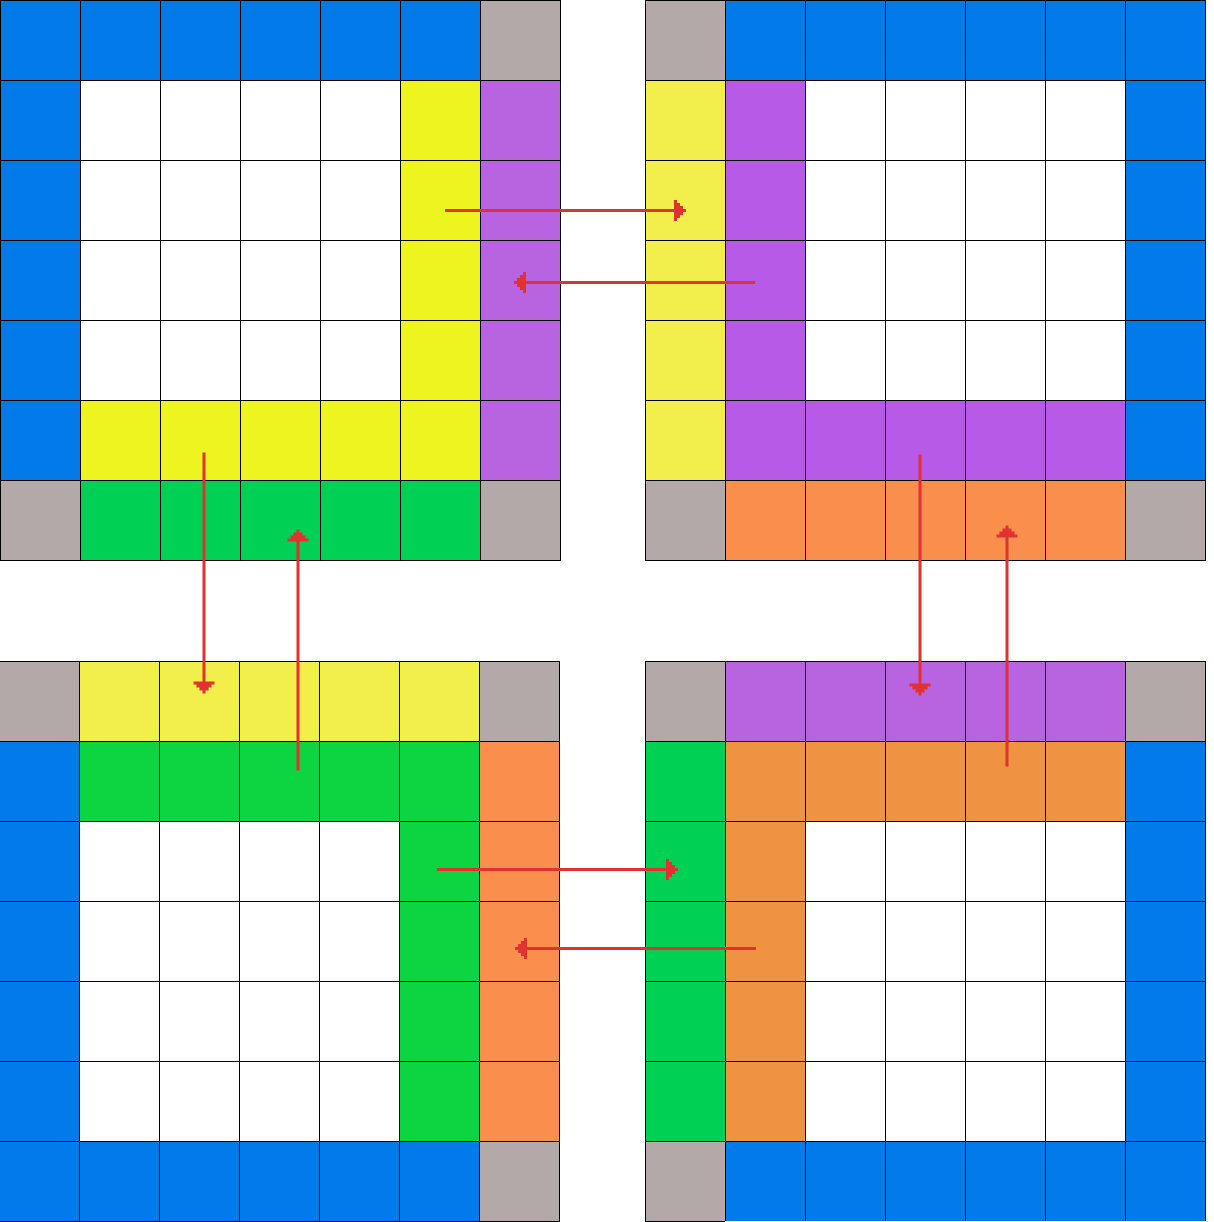
\includegraphics[scale=0.15]{figures/domain-overlap-comms.png}
%  \caption{\label{fig:comms} }
%\end{figure}

%Je m'intéresse ici aux méthodes de communications utilisées dans la première méthode présentée ci-dessus. En effet la seconde méthode d'overlapping n'induit qu'au plus 2 communications par processus par calcul de gradients et ne pose donc pas de problèmes particuliers. En revanche, pour la première méthode il faut effectuer au plus 2x3 communications par appel à la fonction update Sur la figure \ref{fig:neighbor_buf}, on peut voir en orange les ``cellules fantômes'' qui recevront les valeurs voisines et en vert les valeurs qui seront envoyées aux processus voisins. J'ai testé plusieurs de communications pour comparer leurs performance. J'ai dans un premier temps utilisé la fonction MPI\_Neighbor\_alltoallv. Pour l'utiliser, il faut préparer un buffer qui contiendra les données à envoyer à chacun de ses voisins(fig. \ref{fig:neighbor_pos}). La fonction s'occupe elle-même d'envoyer la bonne partie du buffer au bon voisin selon leur disposition sur la grille cartésienne. Après l'appel à cette fonction, le buffer de réception contient les données de tous les voisins autour d'un processus. Il ne reste plus qu'à stocker les variables reçues à leur place. 


\begin{figure}[h!]
  \centering
  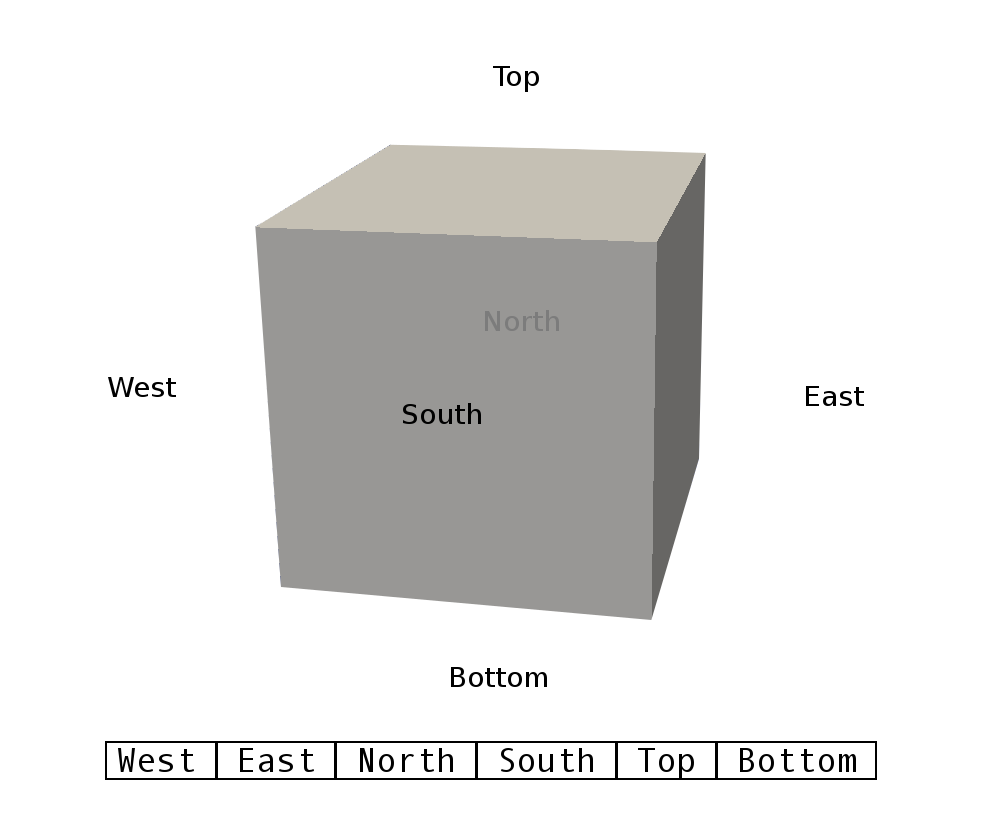
\includegraphics[scale=0.3]{figures/neighbor_pos.png}
  \caption{\label{fig:neighbor_pos}Positions des valeurs des voisins}
\end{figure}

\paragraph{}Cependant cette fonction est relativement récente et peut ne pas être disponible dans les implémentation de MPI présentes sur certains calculateurs qui seront utilisés. Il m'a donc été demandé d'implémenter une seconde méthode dans un soucis de portabilité. C'est une implémentation triviale de la fonction MPI\_Neighbor\_alltoallv; on parcourt les dimensions du domaine, et pour chaque dimension, on effectue 2 envois et 2 réceptions dans la direction correspondant à cette dimension.

%\paragraph{}Le coût d'une telle méthode ne se résume donc pas simplement aux coûts de communications mais aussi aux nombreuses copies réalisées pour créer le buffer d'envoi et pour ``éclater'' le buffer de réception. Ce coût sera donc étudié dans la partie suivante.

%\paragraph{Seconde méthode}
%C'est dans la fonction RHS que les calculs de gradient sont réalisés. Il existe plusieurs méthodes de dérivations selon les propriétés physiques du domaine. C'est dans ses fonctions de dérivations que les communications sont réalisées. Pour chaque méthode de dérivation, il existe 3 fonctions permettant la dérivation sur les 3 axes du domaine. Ces fonctions reçoivent en entrée les valeurs du champ devant être dérivé. Contrairement à la méthode précédente, les communications transmettront moins de donnée (1 seule variable conservative à la fois ici contre les 5 variables plus les espèces dans la première méthode). 

%Il est donc possible de savoir, selon la fonction utilisée, avec quels voisins les communications se feront; par exemple, si la dérivée se fait sur l'axe X (fig. \ref{fig:comm_dim1}), le processus devra réaliser 2 envois et 2 réceptions dans cette direction.  TODO point2point comms




\subsection{Équilibrage de charge}
Lors d'un tel découpage de domaine, il est nécessaire de s'assurer que la quantité de travail réalisée par chaque processus est semblable à celle des autres. Le but est donc de distribuer le même nombre de mailles sur chaque processus. Dans le cas d'un domaine périodique ce problème n'apparaît pas car chaque processus posséde des regions d'overlapping dans toutes les directions. Cependant, si le domaine possède des frontières physique, certains sous-domaines n'auront pas le même besoin d'overlapping.

\paragraph{}Prenons l'exemple d'un domaine de $100\times100\times100$ réparti sur une grille de $4\times4\times4$ processus avec un overlapping de 4: si on découpe le domaine de manière triviale, on obtient donc 64 sous-domaines de taille $25\times25\times25$. Si on ajoute ensuite les points d'overlapping, on retrouve 4 classes de sous-domaines ayant des tailles différentes (fig. \ref{fig:domain_desequilibre}); les coins du domaine auront donc $29\times29\times29$ points (classe C), les autres sous-domaines situés sur les bordures physique auront $33\times29\times29$ points (classe B), les sous-domaines situés sur les faces externes $33\times33\times29$ (classe O) et tous les autres $33\times33\times33$ (classe I). Comme on peut le constater dans le tableau \ref{arr:overlap_res}, la charge de calcul est désiquilibrée entre les processus et certain processus (ceux ayant le moins de travail) devront atteindre les autres pour les synchronisations présentées en début de partie. Même si ce comportement est moins marqué lorsque les sous-domaines sont plus grands (tab. \ref{arr:overlap_res_big}), il est préférable de l'éviter.
  
Si on ajoute la taille totale de l'overlapping avant de découper le domaine, les tailles des domaines internes varient selon les processus mais la taille globale (domaine interne + overlapping) est identique. Toujours avec l'exemple précédent, si on ajoute la taille de l'overlapping à la taille globale, on obtient un domaine global de $124\times124\times124$ points (sur une dimension, les 2 processus se situant aux extrémités possédent 1 seule région d'overlapping tandis que les 2 autres ont eux 2 régions $(2+2+1+1)\times4=24$) . On divise ensuite ce domaine entre les processus et on obtient cette fois-ci une seule classe de sous-domaines de $31\times31\times31$ points. On joue ici sur la taille du domaine interne pour équilibrer la charge. Un sous-domaine se trouvant sur un coin aura un domaine interne de $27\times27\times27$ alors qu'un sous-domaine de classe A aura $23\times23\times23$ point sur son domaine interne.


\begin{figure}[h!t]
  \centering
  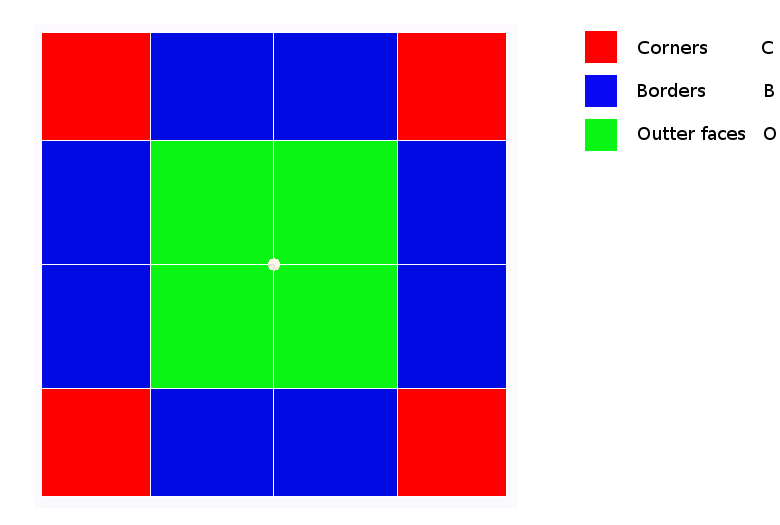
\includegraphics[scale=0.3]{figures/domain_dese.png}
  \caption{\label{fig:domain_desequilibre}Classes de sous-domaines}
\end{figure}

\begin{table}[h!]
  \begin{center}
    \begin{tabular}{|P{2cm}|P{3.5cm}|P{3.5cm}|}
      \hline
      & Taille & Overhead \\ \hline
      C & $29\times29\times29$ & 0\%  \\ \hline
      B & $33\times29\times29$ & 13.8\%  \\ \hline
      O & $33\times33\times29$ & 29.5\%  \\ \hline
      I & $33\times33\times33$ & 47.3\%  \\ \hline      
    \end{tabular}
    \caption{\label{arr:overlap_res}Surcout de calcul - $100\times100\times100$, 64 processus, overlapping 4}
  \end{center}
\end{table}


\begin{table}[h!]
  \begin{center}
    \begin{tabular}{|P{2cm}|P{3.5cm}|P{3.5cm}|}
      \hline
      & Taille & Overhead \\ \hline
      C & $205\times205\times205$ & 0\%    \\ \hline
      B & $210\times205\times205$ & 2.4\%  \\ \hline
      O & $210\times210\times205$ & 4.9\%  \\ \hline
      I & $210\times210\times210$ & 7.5\%  \\ \hline      
    \end{tabular}
    \caption{\label{arr:overlap_res_big}Surcout de calcul - $1000\times1000\times1000$, 125 processus, overlapping 5}
  \end{center}
\end{table}


\paragraph{}Un déséquilibre de charge peut également apparaître lors de la phase d'initialisation, même si son impact peut être faible face à l'ensemble de la simulation, il est préférable de l'éviter. En effet, il faut éviter qu'un seul processus doive initialiser l'ensemble du domaine puis envoyer les informations calculées à tous les autres processus. Dans le cas de ce programme l'initialisation peut-être réalisée de manière indépendante (sans aucune synchronisaton). En effet, les initialisations simples (valeur d'une variable fournie dans le fichier de configuration) ne nécessitent aucun calcul. Les initialisations nécessitant des calculs sont en général basées sur la position physique des points du domaine et peuvent donc être réalisées en totale indépendance.


\subsection{Traitement des bordures internes}
Sur la figure \ref{fig:partdom}, on peut voir que lors du partitionnement du domaine, des bordures internes apparaissent. Ces bordures ne sont donc pas des bordures physique mais des bordure entre sous-domaines et ne doivent pas avoir d'influence sur la simulation. Il ne faut pas appliquer de traitement spécifique aux bordures externes.




Pendant chaque appel à la fonction RHS, les corrections présentées dans la section \ref{sec:nsbc} sont appliquées sur les bordures afin de réduire les instabilitées numériques. Ces corrections sont réalisées par un noyau de calcul qui traite les 2 plans bordure sur chaque direction. Or, il est maintenant possible qu'un sous-domaine possède un seul ou aucun de ces plans. J'ai donc modifié ce noyau afin qu'il ne traite plus qu'un seul plan à la fois, et il n'est appellé que lorsque qu'un processus possède une bordure réelle du domaine. On peut déterminer ceci par rapport à la position des sous-domaines qui est déterminer lors du découpage du domaine.

Des corrections sont également appliquées par rapport à la nature physique des bordure. En effet, différents comportement de frontière sont implémentées dans NTMIX. Ces corrections sont réalisées après chaque appel à RHS. Ce type de correction s'effectuait déjà sur un unique plan mais maintenant seul les sous-domaines avec bordures physique les appliqueront.

%\paragraph{}Seul les processus se trouvant sur les bordure physique du domaine réaliseront donc ces calculs et auront donc une influence sur l'équilibre de charge présenté plus tôt. 

\subsection{Validation}

\paragraph{Cas d'un unique processus}Avant de tester la validité du programme avec plusieurs processus, il est nécessaire de s'assurer qu'il peut être lancé avec un seul processus et que les résulats fournis sont identiques à la version 3D validée à la section \ref{sec:3D-validation}. Même si ce test paraît trivial, il est important de le faire. Il sera également utile de comparer le temps pris par ce test par rapport au temps de la version 3D séquentielle pour estimer le surcôut pouvant être induit par l'utilisation de MPI.

\paragraph{Cas avec décomposition de domaine}
Comme vu dans la section \ref{sec:p2-tr} le calcul des gradients est dépendant de l'ensemble du domaine. Pour s'assurer de l'exactitude des résultats obtenus dans cette version MPI, j'ai donc utiliser un overlapping assez grand permettant d'obtenir une precision numérique suffisante. J'ai ensuite calculer les valeurs moyennes des champs de la solution afin de les comparer avec ceux obtenus avec la version séquentielle du programme (\ref{sec:3D-validation}).

\begin{table}[h]
  \begin{center}
    \begin{tabular}{|c|c|c||c|c|c|c||c|c|c|}
      \hline
      Overlap & 12 & 11 \\
      \hline
      Mean error & 10E-14 & 10E-10 \\
      \hline
    
    \end{tabular}
    \caption{\label{arr:overlap_res} Résultats obtenus}
  \end{center}
\end{table}
